\documentclass{beamer}
\usepackage[utf8]{inputenc}
\usepackage[T1]{fontenc}
\usepackage{url}
\usepackage{hyperref}
\usepackage{minted}
%\usepackage{algorithm2e}
%\usemintedstyle{tango}
\usepackage{xcolor}
%\usepackage[french]{babel}
\usepackage{appendixnumberbeamer}
\usetheme[sectionpage=none,
          subsectionpage=progressbar,
          numbering=fraction,
          progressbar=none,
          background=light]{metropolis}
%\setsansfont[BoldFont={Fira Sans}]{Fira Sans Light}
%\setsansfont[BoldFont={Fira Sans SemiBold}]{Fira Sans Book}
\usefonttheme[onlymath]{serif}

\title{From PCA to Autoencoders}
\subtitle{Unsupervised Representation Learning}
\date{17 décembre 2019}
\author{\textsc{Florent Forest}\vspace{0.2cm}\\
\includegraphics[height=0.35cm]{./rc/e-mail-envelope-blue}\;\scriptsize{\href{mailto:forest@lipn.univ-paris13.fr}{forest@lipn.univ-paris13.fr}}\\
\includegraphics[height=0.35cm]{./rc/grid-world-blue}\;\scriptsize{\href{http://florentfo.rest}{http://florentfo.rest}}\\
\includegraphics[height=0.35cm]{./rc/github-logo-blue}\;\scriptsize{\href{https://github.com/FlorentF9}{FlorentF9}}\\
}
\institute{\vfill\hfill
\includegraphics[height=1.75cm]{./rc/logo_supaero}}

% \newminted{shell}{fontsize=\scriptsize,gobble=4} 
% \newminted{python}{fontsize=\scriptsize,gobble=4,linenos,baselinestretch=0.7}

\begin{document}

  \maketitle

  \begin{frame}{Table of contents}
    \setbeamertemplate{section in toc}[sections numbered]
    %\begin{small}
      %\vspace{0.5cm}
      \tableofcontents%[hideallsubsections]
    %\end{small}
  \end{frame}

  %%%
  \section{Introduction to autoencoders}
  %%%

  \begin{frame}{Motivations}

    \cite{Hinton2006}
    
  \end{frame}

  \begin{frame}{Definition}

    \metroset{block=fill}

    \begin{exampleblock}{Definition}
      \small{
      An \alert{autoencoder} is a neural network trained to reconstruct its inputs. It is composed of two parts:
      \vspace{-0.4cm}
      \begin{enumerate}
        \item an \alert{encoder}, mapping the input to a latent representation ("code") $\mathbf{z} = \mathbf{f}_{\phi}(\mathbf{x})$
        \item a \alert{decoder}, mapping the code back to the input space $\tilde{\mathbf{x}} = \mathbf{g}_{\theta}(\mathbf{z})$
      \end{enumerate}
      }
    \end{exampleblock}

    \begin{figure}
      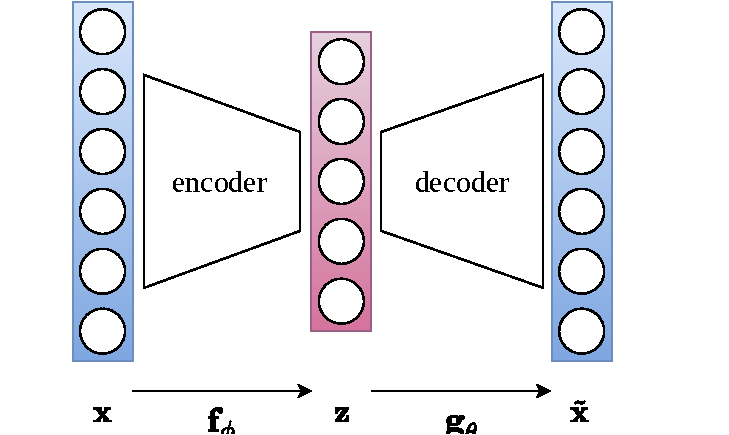
\includegraphics[width=6cm]{rc/autoencoder}
      \caption{Autoencoder architecture}\label{fig:autoencoder}
    \end{figure}

  \end{frame}

  \begin{frame}{Definition}

    \metroset{block=fill}

    \begin{alertblock}{Challenge}
      We do not want the encoder to learn the identity function, but to learn a \emph{good representation} of our data $\rightarrow$ regularization.
    \end{alertblock}

    \vspace{0.5cm}

    \begin{block}{Regularization?}
      Reducing the size of the \emph{hypothesis set} $\mathcal{H}$ by constraining the space of possible solutions to the optimization problem.
      \vspace{-0.4cm}
      \begin{itemize}
        \item L2 weight decay
        \item Sparsity, L1 weight decay
        \item \dots
      \end{itemize}
    \end{block}
    
  \end{frame}

  \begin{frame}{What is a good representation?}

    \metroset{block=fill}
    
    \small{Let $q_{\phi}(Z|X)$ be a (stochastic) mapping from $X$ to $Z$, parameterized by $\phi$. A good representation $Z$ of a random variable $X$ maximizes \alert{mutual information} between $X$ and $Z$:}
    \vspace{-0.4cm}
    \begin{align*}
      \mathbb{I}(X;Z) &= \mathbb{H}(X) - \mathbb{H}(X|Z)\\
                      &= C(X) + \mathbb{E}_{q_{\phi}(X,Z)}\left[\log q_{\phi}(X|Z)\right]
    \end{align*}

    \small{For any parametric distribution $p_{\theta}(X|Z)$ we have $\mathbb{E}_{q_{\phi}(X,Z)}\left[\log p_{\theta}(X|Z)\right] \leq \mathbb{E}_{q_{\phi}(X,Z)}\left[\log q_{\phi}(X|Z)\right]$ (because $D_{KL}(q||p) \leq 0$).}

    \begin{block}{Task: maximize a lower bound on $\mathbb{I}(X;Z)$}
      \begin{equation*}
        \underset{\phi,\theta}{\text{maximize}} \mathbb{E}_{q_{\phi}(X,Z)}\left[\log p_{\theta}(X|Z)\right]
      \end{equation*}
    \end{block}

  \end{frame}

  \begin{frame}{Training autoencoders}

    Loss function for deterministic AE.
    
  \end{frame}

  %%%
  \section{Neurons can learn principal components}
  %%%

  \begin{frame}{Hebb's Learning Rule}

  \end{frame}

  \begin{frame}{Learning PC with Oja's rule}

    \cite{Becker1991}, \cite{Oja1982}, \cite{Oja1992}
    
  \end{frame}

  %%%
  \section{Linear autoencoders}
  %%%

  \begin{frame}{Definition}

    \begin{figure}
      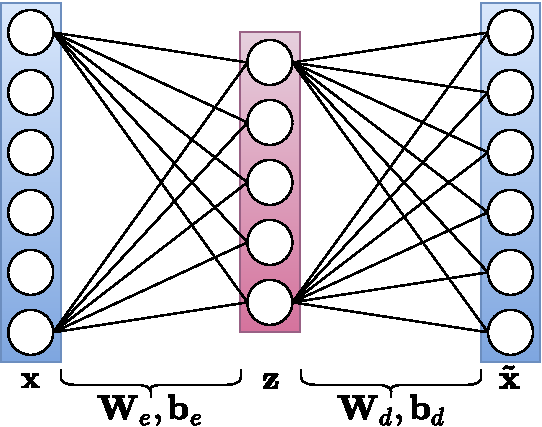
\includegraphics[width=6cm]{rc/linear-autoencoder}
      \caption{Linear autoencoder}\label{fig:linear-autoencoder}
    \end{figure}
    
  \end{frame}

  \begin{frame}{Similarity with PCA}

    \cite{Plaut2018}
    
  \end{frame}

  %%%
  \section{Non-linear autoencoders}
  %%%

  %
  \subsection{Non-linear and deep autoencoders}
  %

  \begin{frame}{Non-linear and deep autoencoders}

    Non-linearity: sigmoid, tanh, ReLU\dots

    Several layers

    Layer-wise pretraining: \cite{Hinton2006}
    In fact, not necessary (source?).
    
  \end{frame}

  %
  \subsection{Different types of regularization}
  %

  \begin{frame}{Undercomplete or overcomplete}
    
  \end{frame}

  \begin{frame}{Let's code!}

    % AE classique avec une/plusieurs couches
    % Éventuellement convolutif
    % Mettre en évidence l'overfitting (1 code par point) avec un exemple
    
  \end{frame}

  \begin{frame}{Sparse autoencoders}
    
  \end{frame}

  \begin{frame}{Denoising autoencoders}

    \cite{Vincent2010}
    
  \end{frame}

  \begin{frame}{Variational autoencoders (VAE)}
    
    \cite{Kingma2014}

    % Lien vers le blog VAE, utiliser des images

    See also litterature on GAN.

  \end{frame}

  \begin{frame}{Let's code!}

    % VAE
    
  \end{frame}

  %%%
  \section{Applications}
  %%%

  \begin{frame}{Feature extraction}

    Dimensionality reduction, useful features

    Pre-processing pour d'autres algos (regress, classif, clustering)
    
  \end{frame}

  \begin{frame}{Unsupervised pretraining for supervised learning}
    
    Unsupervised pretraining -> supervised finetuning

    \cite{Erhan2010}

  \end{frame}

  \begin{frame}{Visualization}
    
  \end{frame}

  \begin{frame}{Data compression}
    
    Dimensionality reduction
    Data-specific, lossy compression.

  \end{frame}  

  \begin{frame}{Data augmentation}

    Noise/interpolation/extrapolation in feature space \cite{Devries2017}.

    Generative models (VAE, GAN).

  \end{frame}

  \begin{frame}{Anomaly detection}
    
    L'erreur de reconstruction peut être utilisée comme un score d'anomalie.

  \end{frame}

  %%%
  \appendix

  \begin{frame}[allowframebreaks]{References}
    
    \bibliography{references}
    \bibliographystyle{abbrv}
  
  \end{frame}

\end{document}